\section{Cookie Banner: Manipulativ?}
\subsection{Einleitung in das Beispiel}
Internetseiten nutzen zum Anzeigen und Senden von Daten das sogenannte \ac{HTTP}. Bei \ac{HTTP} handelt es sich um ein sogenanntes ``stateless'' (zustandsloses) Protokoll, d.h. alle Anfragen und Transaktionen zwischen dem Nutzer und der aufgerufenen Internetseite sind unabhängig voneinander. Dadurch fällt es schwer, Zusammenhänge und Nutzerdaten mehrerer Anfragen mitzusenden und abrufbar zu halten.

Cookies werden eingesetzt, wenn bestimmte Infos zwischen mehreren Anfragen gespeichert werden sollen. Sie sind kleine Dateien, welche von der aufzurufenden Internetseite angefordert und gesendet werden. Die Cookies werden dann vom genutzten Internetbrowser angelegt und verwaltet. Sie sind dabei immer spezisich für die Seite, die sie anfragt und sendet und werden genutzt, um beispielsweise Internetseiten mit Kontofunktionen zu realisieren. \footfullcite[S. 4-6]{Kristol.}

\subsection{Problemstellung}
Obwohl Cookies spezifisch für jede Internetseite sind und ein Verknüpfen von Nutzerdaten über mehrere Internetseiten hinweg nicht möglich sein sollte, wurde durch die Funktionsweise des Internets schnell eine Möglichkeit gefunden, Cookies für mehrere Seiten zu nutzen.

Dabei wird neben der gewünschten Internetseite noch eine weitere Seite geladen, welche den Cookie setzt und anfordert. Wenn dieses System über mehrere Internetseiten hinweg genutzt wird, können die Interessen eines Nutzers nachverfolgt werden. Man spricht hierbei vom ``Third Party Cookies'', da das Datensammeln nicht direkt durch den Seitenbetreiber selbst passiert. \footfullcite[S. 2608]{Bielova.2017}

\begin{figure}[ht]
	\centering
	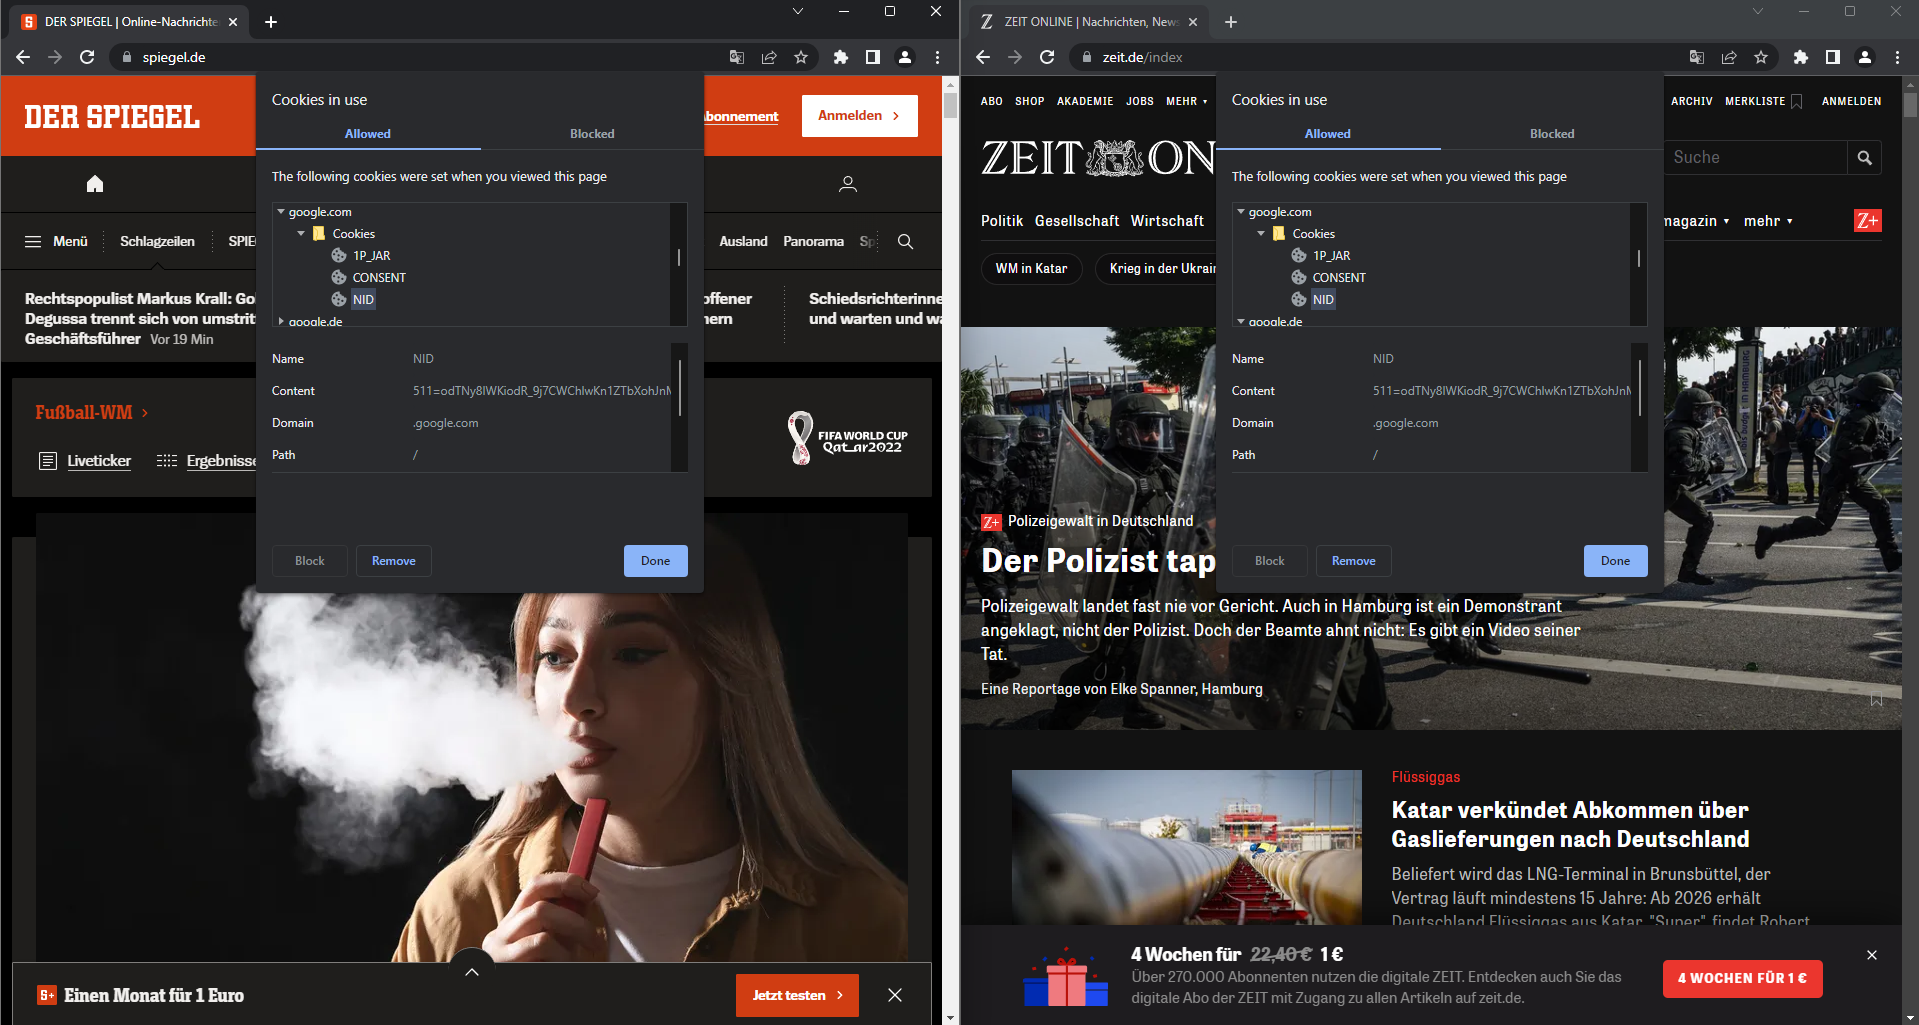
\includegraphics[width=1\textwidth]{Bilder/Cookies.png} 
	\caption{Ein Third Party Cookie, welcher bei Spiegel und Zeit genutzt wird}
	\label{fig:Third-Party}
\end{figure}

Durch Verabschiedung der \ac{DSGVO} in der \ac{EU} im Jahr 2016 \footfullcite{EuropaischeUnion.2016} gibt es für Cookies in der \ac{EU} einen rechtlichen Rahmen zur Verwendung jener. Dieser sieht vor, dass lediglich ``First Party Cookies'', also Cookies, welche direkt von der aufgerufenen Internetseite erstellt werden, genutzt werden dürfen. Entsprechenden ``Third Party Cookies'', welche hauptsächlich zum Sammeln von Nutzerdaten genutzt werden, muss der Nutzer nach der \ac{DSGVO} erst explizit zustimmen. Die \ac{EU} erhofft sich davon mehr Transparenz im Bezug auf die Verarbeitung personenbezogener Daten. \footfullcite[S. 84]{EuropaischeUnion.2016}

Unternehmen ist in vielen Fällen jedoch daran gelegen, möglichst viele ``Third Party Cookies'' einzubinden. So gibt es ganze Geschäftsmodelle, welche Cookies zu Werbe- und Analysezwecken nutzen und durch das effektive Sammeln und Auswerten von Daten Umsatz generieren.\footfullcite[S. 418-420]{.2012} Durch die gegebenen Umstände entwickelte sich so der Trend, dass zur Einwilligung in die Datensammlung ein Nudge genutzt wird, welcher die Entscheidung beeinflussen soll.

\subsection{Aufbau und Wirkung}
Die Zustimmung zu Cookies wird auf Internetseiten meist in Form eines Banners realisiert, welcher den Nudge enthält. Der Cookie Banner fragt dabei den Nutzer, ob das Einsetzen von Drittanbieter Cookies und damit das Sammeln von Daten gestattet ist. Die Gestaltung weicht dabei je nach Plattform stark voneinander ab.

\begin{figure}[ht]
    \centering
    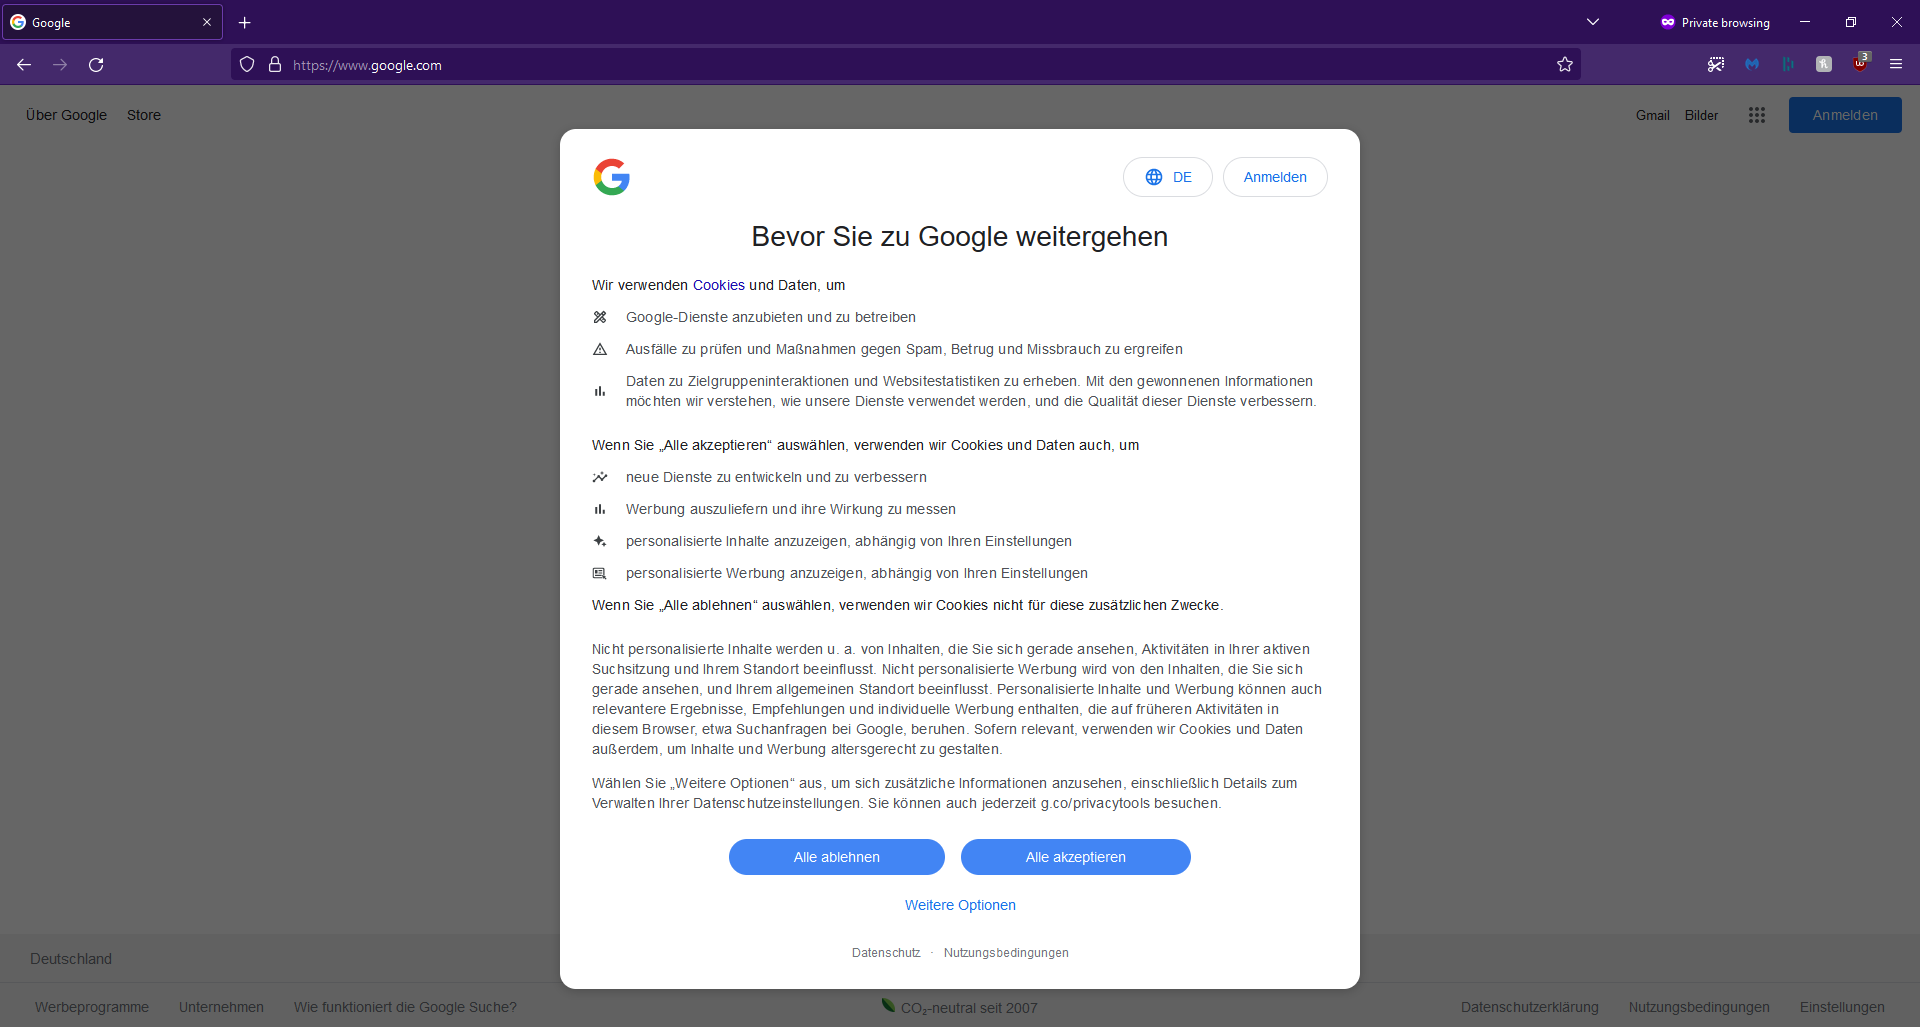
\includegraphics[width=1\textwidth]{Bilder/Google_Banner.png}
    \caption{Cookie Banner auf www.google.com}
    \label{fig:Google-Cookie}
\end{figure}

Beim ersten Aufrufen der Website \url{https://www.google.com} wird der Cookiebanner angezeigt. Dabei wird bereits direkt ein Nudge auffällig. Der Banner wird zentral über dem eigentlichen Inhalt des Bildschirms platziert. Der Nutzer, welcher gerade etwas bei Google suchen möchte, muss daher zuerst mit dem Banner interagieren. Google bietet hier einen Knopf ``Alles Akzeptieren'' und ``Alles ablehnen'' an. Dennoch wird hier bereits Einfluss auf den Nutzer genommen, da sein Nutzungserlebnis direkt gestört wird und er erst einen der beiden Knöpfe drücken muss, um mit seiner Arbeit fortzufahren.

Auf der Webseite von Facebook (\url{https://www.facebook.com/de}) wird neben dem inhaltsverdeckenden Banner ein weiterer Nudge eingesetzt. Die Option ``Erforderliche und optionale Cookies erlauben'' ist in einem auffälligen Blau markiert, während die Option ``Nur erforderliche Cookies erlauben'' in einer grauen Farbe gezeigt wird.

\begin{figure}[ht]
    \centering
    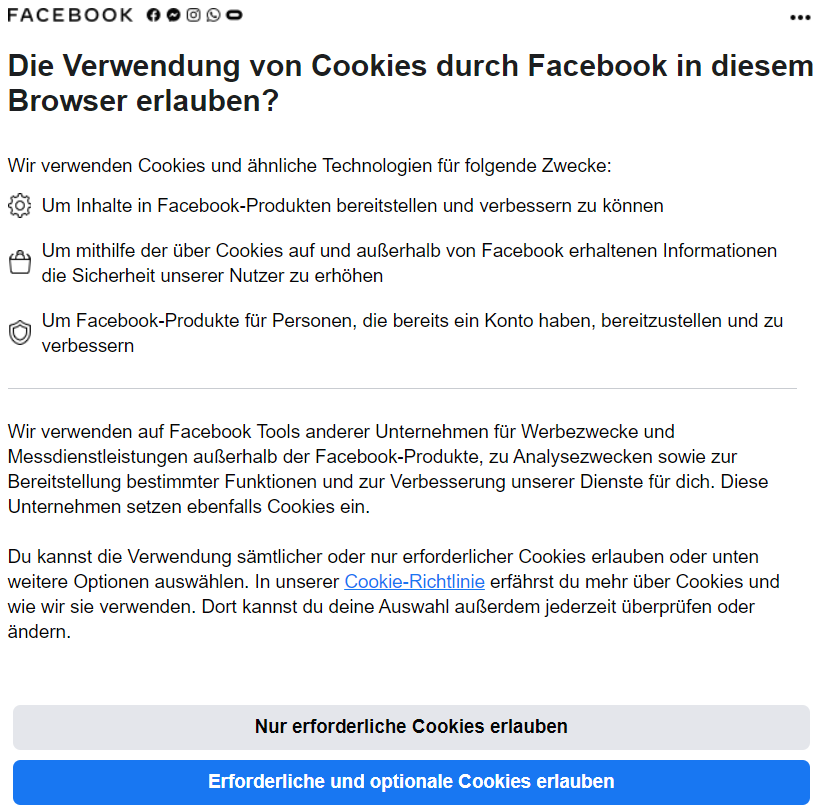
\includegraphics[width=0.8\textwidth]{Bilder/Facebook_Banner.png}
    \caption{Cookie Banner auf www.facebook.com mit farblich unterschiedlichen Knöpfen}
    \label{fig:Facebook-Cookie}
\end{figure}

Die farbliche Hervorhebung einer Option erscheint für den Nutzer hierbei wie eine Empfehlung und sticht mehr ins Auge, als der hellgraue Farbton, welcher sehr ähnlich zum Hintergrund wirkt. Hervorhebung einer gewünschten Option kann nicht nur durch Farbe, sondern auch durch Positionierung und Größe innerhalb des Banners passieren.

Eine weitere Möglichkeit, den Nutzer in seiner Entscheidung zu beeinflussen, stellt das Verlagern der Ablehnen Funktion auf eine Extra Seite dar. Hierbei wird dem Nutzer lediglich eine Option zum Akzeptieren und eine Option zum Ansehen diverser Einstellungen bezüglich des Datenschutzes angeboten.

\begin{figure}[ht]
    \centering
    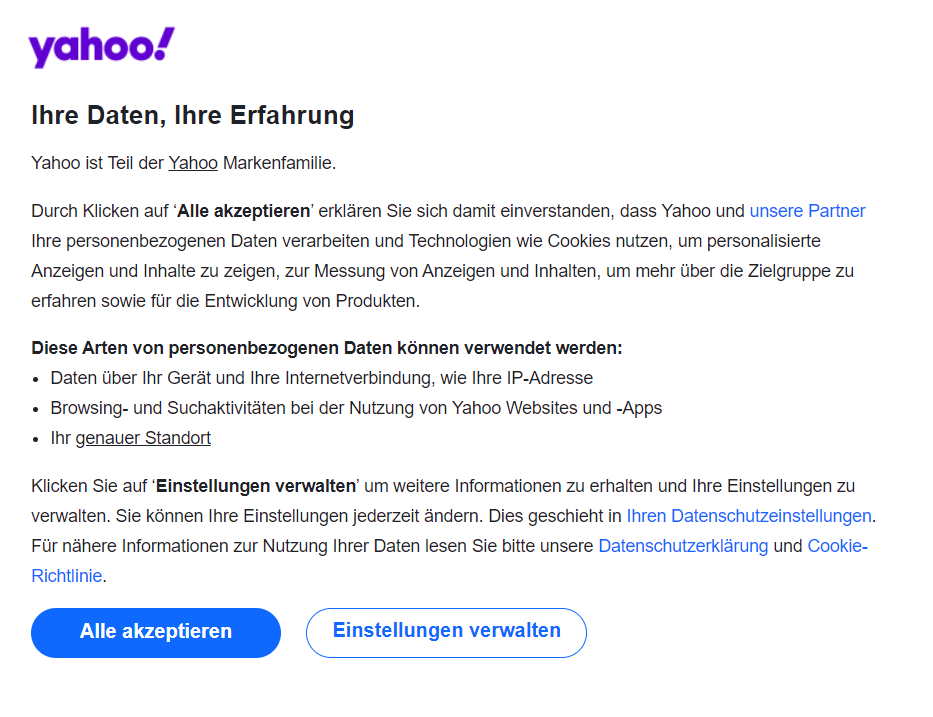
\includegraphics[width=0.8\textwidth]{Bilder/Yahoo_Banner.png}
    \caption{Cookie Banner auf www.yahoo.de mit Einstellungsknopf}
    \label{fig:Yahoo-Cookie}
\end{figure}

Dieses Verlagern der Ablehnenfunktion auf eine weitere Seite ist besonders effektiv, wenn der Nudge dazu genutzt werden soll, dass Nutzer tendenziell dem Datensammeln zustimmen. Die Zustimmung aller Cookies ist 22 - 23 \% wahrscheinlicher, wenn die Ablehnenfunktion nicht direkt im Banner enthalten ist. \footfullcite[S. 8]{Nouwens.2020}

\subsection{Bewertung anhand der ethischen Grundlagen}

Je nach Funktionsweise lässt sich nachweisen, dass die hier gezeigten Beispiele gegen die in Kapitel HIER EINSETZEN verstoßen.
Während die Einblendung von Google (siehe Abbildung \ref{fig:Google-Cookie}) mit den Optionen ``Alles Akzeptieren'' und ``Alles ablehnen'' eine transparente und autonome Auswahl der Einstellungen ermöglicht, lässt sich argumentieren, dass die Banner von Facebook (siehe Abbildung \ref{fig:Facebook-Cookie}) und Yahoo (siehe \ref{fig:Yahoo-Cookie}) gegen ethische Grundsätze von digitalen Nudges verstoßen.

In beiden Fällen ist die Transparenz eingeschränkt, da eine Option (Alles akzeptieren) farblich hervorgehoben ist und die Wahl damit nicht mehr neutral ist. Yahoo geht außerdem einen Schritt weiter und bietet gar nicht mehr alle Optionen direkt an (``Alles ablehnen''), sondern versteckt den Inhalt auf einer Einstellungsseite, was nicht nur Transparenz sondern auch Autonomie einschränkt.

Deutsche Zeitungsanbieter nutzen dieses Prinzip und bieten keine Option zum Ablehnen mehr an. Hier wird lediglich vorgeschlagen, die Cookierichtlinien zu akzeptieren oder für ein cookiefreies Modell zu bezahlen.

\begin{figure}
    \centering
    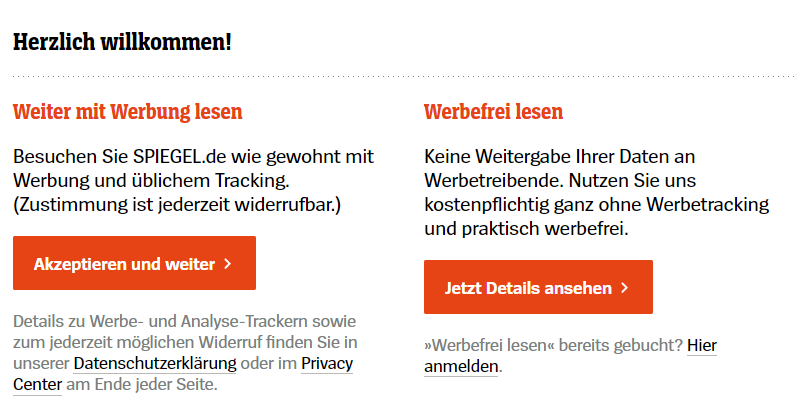
\includegraphics[width=0.9\textwidth]{Bilder/Spiegel_Banner.png}
    \caption{Cookie Banner auf www.spiegel.de mit Bezahlfunktion}
    \label{fig:Spiegel-Cookie}
\end{figure}

Hier sind Autonomität und Transparenz noch eingeschränkter, da gar nicht mehr alle Optionen (Cookies ablehnen) angeboten werden. Dem Nutzer wird lediglich angeboten, alle Cookies zu akzeptieren, eine Option alles abzulehnen gibt es nicht mehr.

Abschließend lässt sich sagen, dass die Nutzung von Cookie Bannern bei bekannten Plattformen klar gegen ethische Grundlagen verstößt. Neben den Idealen der Autonomität und Transparenz, verstoßen alle genannten Beispiele auch gegen den Grundsatz der Zielrechtfertigung, da mit dem Aktivieren der Cookies weder soziale noch nutzerfreundliche und lediglich Interessen der Plattform verfolgt werden. Auch rechtlich sind die gezeigten Beispiele bereits kritisiert worden. So verurteilte die französische Datenschutzbehörde Facebook und Google zu hohen Geldstrafen aufgrund von Verstößen gegen die DSGVO im Bezug auf die Implementierung von Cookie-Bannern. \footfullcite{AnnaBiselli.2022}